\documentclass[border=2pt]{standalone}
\usepackage{pgfplots}
\pgfplotsset{compat=1.18}
\definecolor{red}{rgb}{0.7,0.11,0.11}
\definecolor{blue}{rgb}{0.0,0.20,0.42}
\definecolor{green}{rgb}{0.11,0.35,0.02}
\begin{document}
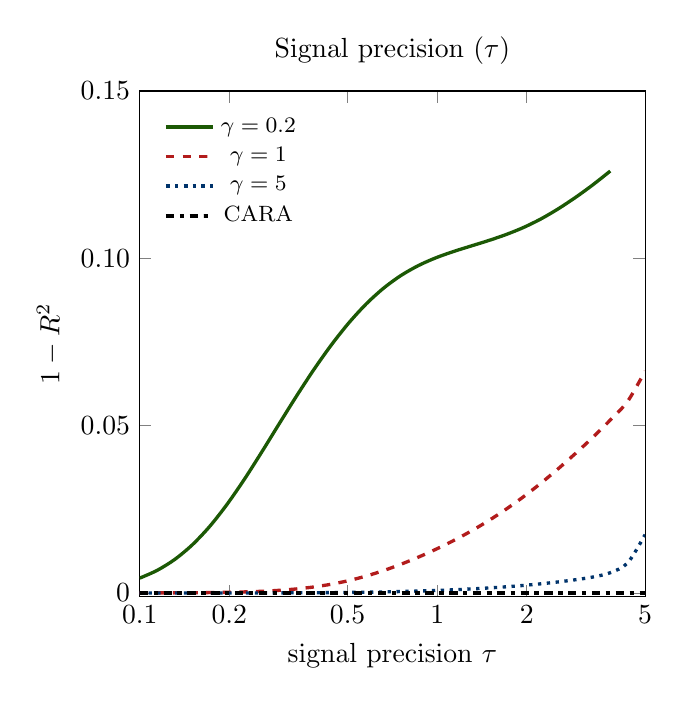
\begin{tikzpicture}
\begin{axis}[
    width=8cm, height=8cm,
    xmode=log,
    xmin=0.1, xmax=5,
    ymin=-0.001, ymax=0.15,
    xtick={0.1,0.2,0.5,1,2,5},
    xticklabels={0.1,0.2,0.5,1,2,5},
    ytick={0,0.05,0.1,0.15},
    yticklabels={0,0.05,0.10,0.15},
    xlabel={signal precision $\tau$},
    ylabel={$1 - R^2$},
    title={Signal precision ($\tau$)},
    legend pos=north west,
    legend style={fill=none, draw=none, font=\footnotesize},
    smooth,
]
\addplot[very thick, color=green, smooth] coordinates {(0.1,0.00444395) (0.114442,0.00675354) (0.13097,0.00998458) (0.149884,0.0143021) (0.17153,0.0197866) (0.196303,0.0263916) (0.224652,0.0339291) (0.257097,0.0420933) (0.294226,0.0505184) (0.336718,0.0588494) (0.385347,0.0667948) (0.440998,0.0741348) (0.504687,0.0807024) (0.577573,0.0863763) (0.660986,0.0910979) (0.756445,0.0948886) (0.865691,0.0978519) (0.990713,0.100158) (1.13379,0.102018) (1.29753,0.103652) (1.48492,0.105269) (1.69937,0.107052) (1.94479,0.109151) (2.22566,0.111698) (2.54709,0.114729) (2.91494,0.118165) (3.33591,0.121945) (3.81768,0.126061)};
\addplot[very thick, color=red, dashed, smooth] coordinates {(0.1,1.62471e-05) (0.114442,2.72258e-05) (0.13097,4.5383e-05) (0.149884,7.51571e-05) (0.17153,0.000123469) (0.196303,0.000200853) (0.224652,0.000322852) (0.257097,0.000511529) (0.294226,0.000796661) (0.336718,0.00121589) (0.385347,0.0018128) (0.440998,0.0026319) (0.504687,0.00371055) (0.577573,0.00506967) (0.660986,0.00670784) (0.756445,0.00860406) (0.865691,0.0107311) (0.990713,0.0130731) (1.13379,0.015637) (1.29753,0.0184498) (1.48492,0.0215451) (1.69937,0.0249494) (1.94479,0.0286752) (2.22566,0.0327186) (2.54709,0.0370607) (2.91494,0.0416697) (3.33591,0.0465004) (3.81768,0.0516664) (4.36903,0.0572715) (5,0.0662943)};
\addplot[very thick, color=blue, dotted, smooth] coordinates {(0.1,8.50445e-07) (0.114442,1.39006e-06) (0.13097,2.25716e-06) (0.149884,3.63844e-06) (0.17153,5.81783e-06) (0.196303,9.22057e-06) (0.224652,1.44726e-05) (0.257097,2.24769e-05) (0.294226,3.45056e-05) (0.336718,5.22977e-05) (0.385347,7.81402e-05) (0.440998,0.000114891) (0.504687,0.000165889) (0.577573,0.000234722) (0.660986,0.000324868) (0.756445,0.000439402) (0.865691,0.000581011) (0.990713,0.000752524) (1.13379,0.000957802) (1.29753,0.00120247) (1.48492,0.00149395) (1.69937,0.00184083) (1.94479,0.00225185) (2.22566,0.00273517) (2.54709,0.00329822) (2.91494,0.00395493) (3.33591,0.00476692) (3.81768,0.00605046) (4.36903,0.00898551) (5,0.0174295)};
\addplot[ultra thick, color=black, dashdotted]
    coordinates {(0.1,0)(5,0)};
\addlegendentry{$\gamma = 0.2$}
\addlegendentry{$\gamma = 1$}
\addlegendentry{$\gamma = 5$}
\addlegendentry{CARA}
\end{axis}
\end{tikzpicture}
\end{document}
